%%%%%%%% ICML 2018 EXAMPLE LATEX SUBMISSION FILE %%%%%%%%%%%%%%%%%

\documentclass{article}

% Recommended, but optional, packages for figures and better typesetting:
\usepackage{microtype}
\usepackage{graphicx}
\usepackage{subfigure}
\usepackage{booktabs} % for professional tables
\usepackage{url}
\usepackage{cite}
\usepackage{subfigure}
\usepackage{amsmath} 
\usepackage{amsfonts}
\usepackage{amssymb,bm}
 

% hyperref makes hyperlinks in the resulting PDF.
% If your build breaks (sometimes temporarily if a hyperlink spans a page)
% please comment out the following usepackage line and replace
% \usepackage{icml2018} with \usepackage[nohyperref]{icml2018} above.
\usepackage{hyperref}

% Attempt to make hyperref and algorithmic work together better:
\newcommand{\theHalgorithm}{\arabic{algorithm}}

% Use the following line for the initial blind version submitted for review:
\usepackage{icml2018}

% If accepted, instead use the following line for the camera-ready submission:
%\usepackage[accepted]{icml2018}

% The \icmltitle you define below is probably too long as a header.
% Therefore, a short form for the running title is supplied here:
\icmltitlerunning{Submission and Formatting Instructions for ICML 2018}

\begin{document}

\twocolumn[
\icmltitle{Submission and Formatting Instructions for \\
           International Conference on Machine Learning (ICML 2018)}

% It is OKAY to include author information, even for blind
% submissions: the style file will automatically remove it for you
% unless you've provided the [accepted] option to the icml2018
% package.

% List of affiliations: The first argument should be a (short)
% identifier you will use later to specify author affiliations
% Academic affiliations should list Department, University, City, Region, Country
% Industry affiliations should list Company, City, Region, Country

% You can specify symbols, otherwise they are numbered in order.
% Ideally, you should not use this facility. Affiliations will be numbered
% in order of appearance and this is the preferred way.
\icmlsetsymbol{equal}{*}

\begin{icmlauthorlist}
\icmlauthor{Christopher Krolla}{equal,fr}
\icmlauthor{Thomas Nierhoff}{equal,fr}
\icmlauthor{Philipp Yankov}{equal,fr}
\end{icmlauthorlist}

\icmlaffiliation{fr}{University of Freiburg, Freiburg, Germany}

\icmlcorrespondingauthor{Cieua Vvvvv}{c.vvvvv@googol.com}
\icmlcorrespondingauthor{Eee Pppp}{ep@eden.co.uk}

% You may provide any keywords that you
% find helpful for describing your paper; these are used to populate
% the "keywords" metadata in the PDF but will not be shown in the document
\icmlkeywords{Machine Learning, ICML}

\vskip 0.3in
]

% this must go after the closing bracket ] following \twocolumn[ ...

% This command actually creates the footnote in the first column
% listing the affiliations and the copyright notice.
% The command takes one argument, which is text to display at the start of the footnote.
% The \icmlEqualContribution command is standard text for equal contribution.
% Remove it (just {}) if you do not need this facility.

%\printAffiliationsAndNotice{}  % leave blank if no need to mention equal contribution
\printAffiliationsAndNotice{\icmlEqualContribution} % otherwise use the standard text.


%%%%%%%%%%%%%%%%%%%%%%%%%%%%%%%%%%%%%%%%%%%%%%%%%%%%%%%%%%%%%%%%%%%%%%%%%%%%%%%%
\begin{abstract}
Abstract
\end{abstract}




%%%%%%%%%%%%%%%%%%%%%%%%%%%%%%%%%%%%%%%%%%%%%%%%%%%%%%%%%%%%%%%%%%%%%%%%%%%%%%%%
\section{Introduction}
Machine learning (ML) is a fast-growing field in the domain of computer science, most notably neural networks. Instead of manually tweaking the features used for classification or regression, neural networks are able to extract them automatically. They have shown state-of-the-art performance on a variety of classification problems when trained on huge datasets and run on large computing clusters. 

A open question is how to deal with computational limitations and generic datasets. In many real-world applications (e.g. smartphones) computational resources, execution time and storage capacity is limited. Thus the current trend of using larger and larger networks for better classification results becomes unfeasible. Different approaches emerged within the last years to tackle the challenge: 

To reduce the model size (and thus implicitly also execution time, storage capacity and computational resources), one can simply remove the most ``unimportant'' parts of a neural network and/or quantize it, resulting in a compression of the neural network The selection of the nodes/layers to be pruned can either be specified manually or derived automatically through reinforcement learning~\cite{han15,han18}. Another option is knowledge distillation where a smaller student``network'' is trained to produce outputs similar to a previously trained larger ``teacher'' network~\cite{hinton15,phuong19}. By using the logits output instead of the softmax output, much more information is preserved in every training step. Thus training the student network can be achieved with way less samples. For both approaches there is only a negligible decrease in classification accuracy while the compression rate can be huge (up to a factor of 496x for certain layers of a neural network ~\cite{reagan18}). Another more straightforward method is to search directly for smaller/faster models. This can be either done manually (e.g.~\cite{howard17}) or through neural architecture search~\cite{elsken18}. Note that the last approach can output networks that are state of the art with respect to model size, speed and classification accuracy~\cite{tan19}.

Other techniques are used if the time budget for training is tight or the dataset to be trained is small. They all have in common that a network is pretrained on one or more datasets beforehand and information from pretraining is subsequently used for the final training step. One common technique is transfer learning~\cite{pan10}. Here the common use case consists of pretraining a network on a given dataset to initialize the network weights with reasonable values. If a new dataset is similar enough, only parts of the network must be trained again. In addition, the new dataset can be rather small as less optimization steps are required (the network is not trained from scratch). Another option is meta-learning or learning to learn~\cite{santoro16,hutter19}: By learning multiple models for multiple tasks (or more specific: datasets) beforehand, it is quite likely that a new task will be similar to a previously learned task. In this case, knowledge gained from the previous task can be reused, thus accelerating the learning progress. The challenge with meta-learning is a proper selection of the meta-features to be extracted as their predictive capabilities vary heavily~\cite{bilalli17}
One predominant meta-learning approach at the moment is MAML \cite{finn17}, optimizing a model not for classification accuracy but specifically for generalization performance. 

The AutoDL challenge contains both aspects, tight computational limitations (both time- and resource-wise) and generic datasets. As such it provides an ideal testbed for advanced approaches in order to find data-savvy and time-efficient algorithms. Because the datasets are undisclosed, the options for manual tweaking are limited. Instead of highly specific solutions tied to a specific environment one is thus seeking for a fast yet robust approach. This makes the challenge different from ``traditional'' benchmarks like ImageNet classification rate where computing power is solely limited by the budget of the chair/institute and the dataset is given a priori. 

The remainder of the paper is organized as follows: Sec.~\ref{sec:problem} describes the general problem from a more mathematical point of view. Sec.~TODO provide general background information about the AutoDL challenge, the used datasets and initial approaches for the AutoDL video competition. As focus shifted after the video competition, Sec.~TODO illustrates two more elaborate approaches for video and image classification that can be used for the final AutoDL challenge. 

%%%%%%%%%%%%%%%%%%%%%%%%%%%%%%%%%%%%%%%%%%%%%%%%%%%%%%%%%%%%%%%%%%%%%%%%%%%%%%%%%
\section{Problem formulation}
\label{sec:problem}



%%%%%%%%%%%%%%%%%%%%%%%%%%%%%%%%%%%%%%%%%%%%%%%%%%%%%%%%%%%%%%%%%%%%%%%%%%%%%%%%%
\section{AutoDL challenge}
\label{sec:autodl}
This section gives a quick overview of the AutoDL challenge: The AutoDL challenges consist of a set of different, individual challenges depending on the underlying dataset modality: Image (AutoCV), video (AutoCV2), text (AutoNLP), speech (AutoSpeech), weakly supervised learning (AutoWSL) and everything together (AutoDL). 
All challenges have in common that teams can upload code with their models during a online phase which is tested immediately on a number of datasets. This gives every team a good feedback about their relative performance. These online phases last between two weeks and two months. Some challenges (e.g. for video) have a second, full blind testing (onsite) phase at the end where every team's last submission is evaluated on a new, previously unknown set of of datasets. 

Differing from other challenges, there were rather tight constraints: Rather than focusing on the final classification accuracy after a certain time limit, each team can choose freely how much time to spend on training and how much on testing within a specific time budget $T=1200s$. Training is performed by running a ``train'' function with the train dataset as input, test by running a ``test'' function with the test dataset as input and the classification results as output. Based on the output of every test run its score $s(t)$ at time $t$ is calculated as 
%
\begin{equation}
s(t) = 2*AUC - 1, \nonumber
\end{equation} 
%
with $AUC$ as the area under receiver operating characteristic curve. The final score $ALC$ is then calculated as the time integral over all individual scores $s(t)$, weighted on a logarithmic time scale as
%
\begin{equation}
ALC = \frac{1}{\log \left( 1 + \frac{T}{t_0} \right)} \int_0^T \frac{s(t)}{t+t_0} dt, \nonumber
\label{eq:ALC}
\end{equation} 
%
with $t_0=20s$. This way, the predictions of every test run at time $t$ are weighted with $\frac{1}{t+t_0}$. Because early predictions are weighted more, focus shifts from a high classification accuracy at the end of the time budget to a high accuracy as early as possible. A example of $ALC$ can be seen in Fig.~\ref{fig:learningCurveExample}. It is visible that the performance within the first $60s$ counts roughly as much as the performance within the last $600s$.
%
\begin{figure}[htb]
\begin{center}
 	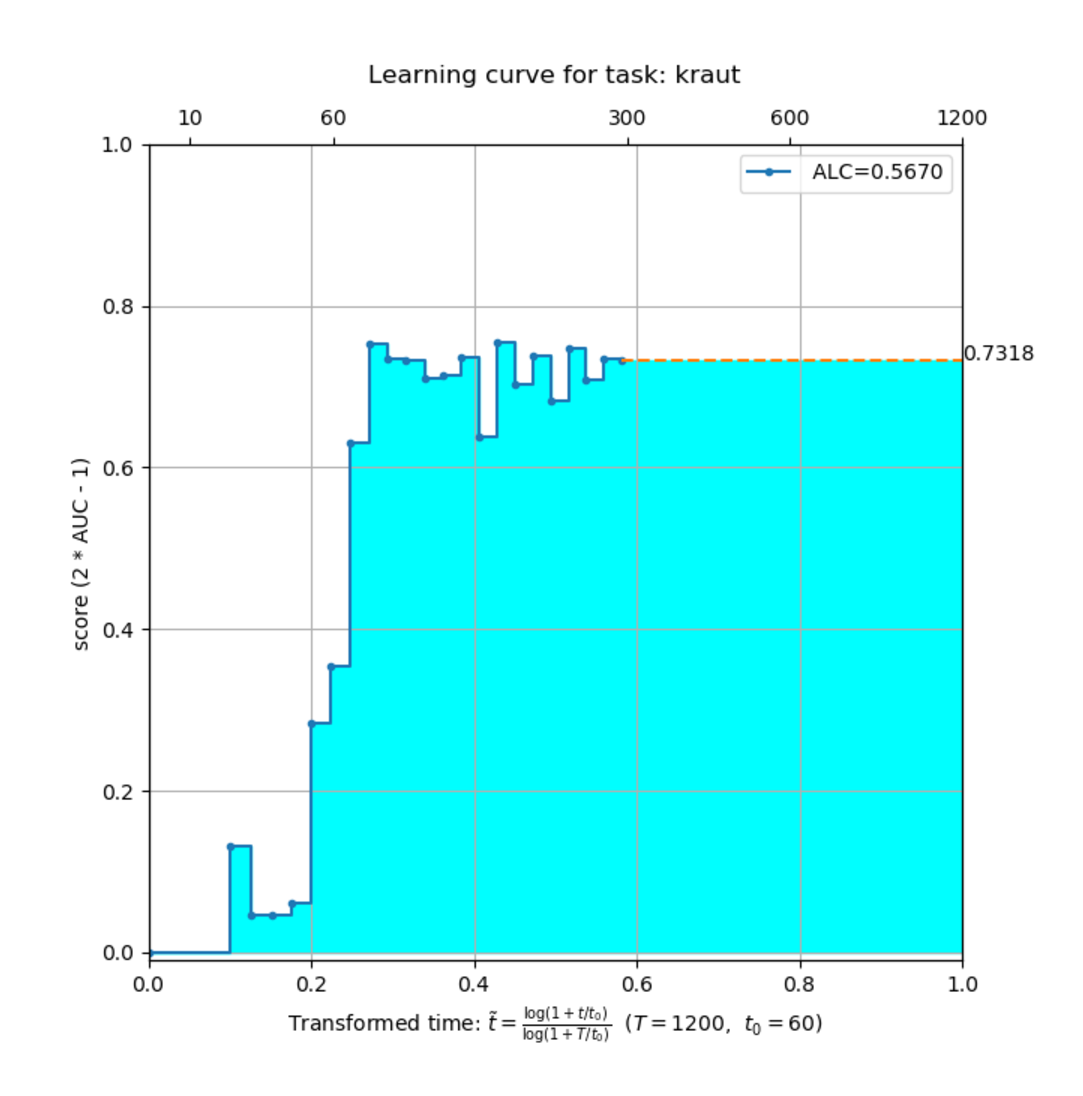
\includegraphics[width=0.95\linewidth]{../figures/learning-curve-example.eps} 
\end{center}
\caption{Visualization of the ALC plotted over time}
\label{fig:learningCurveExample}
\end{figure} 
%
Additional limitations consider memory constraints (max. 300Mb per submission), computational constraints (NVIDIA Tesla P100 1GPU, 4vCPU, 26GB) and time constraints (AutoCV2: max. 5 hours runtime per 24 hours, max. 5 submissions per 24 hours).


%%%%%%%%%%%%%%%%%%%%%%%%%%%%%%%%%%%%%%%%%%%%%%%%%%%%%%%%%%%%%%%%%%%%%%%%%%%%%%%%%
\section{Datasets}
\label{sec:datasets}
Below is an table of the datasets used for training our models. Shown is the dataset name both for image and video datasets, the number of train samples, test samples and classes and the source from where the dataset can be obtained. Datasets marked with ``tfds'' can be obtained using the Tensorflow Datasets module, the ones marked with ``AutoDL'' using the provided code from the AutoDL challenge and the ones with ``inet'' are publicly available. Both the Youtube8m and YFCC100m have been downloaded partially by using/extracting the individual video links in/from the dataset file. Note that these two datasets are also the only two multilabel datasets.
Although looking promising in theory as they are both the largest video datasets available and the only multilabel datasets used, Youtube8m and YFCC100m were impossible to use due to their sheer size. Even if the exact reason is unknown (possible inode overhead due to many files), training any neural network on them is unfeasible slow TODO.
Furthermore, results from the AutoCV2 challenge indicate that it is in general unnecessary to capture multiple frames from a video (one is sufficient), thus turning the video classification task into a image classification task.

\begin{table}
\center
\tiny 
\begin{tabular}{|l|r|r|r|r|}
\hline
image dataset name & train samples & test samples & classes & source \\
\hline
Binary Alphadigits & 1115 & 289 & 36 & tfds \\
Caltech101 & 3059 & 6085 & 102 & tfds \\
CUB-200 & 3000 & 3033 & 200 & tfds \\
CUB-200-2011 & 5994 & 5794 & 200 & tfds \\
Cats and Dogs & 22263 & 999 & 2 & tfds \\
CIFAR-10 & 50000 & 10000 & 10 & tfds \\
CIFAR-100 & 50000 & 10000 & 100 & tfds \\
COIL-100 & 6202 & 998 & 72 & tfds \\
Colorectal Histology & 4003 & 997 & 8 & tfds \\
DeepWeeds & 16520 & 989 & 5 & tfds \\
EuroSAT & 25976 & 1024 & 10 & tfds \\
EMNIST & 697932 & 116323 & 62 & tfds \\
Fashion-MNIST & 60000 & 10000 & 10 & tfds \\
Horses or Humans & 1027 & 256 & 2 & tfds \\
KMNIST & 60000 & 10000 & 10 & tfds \\
MNIST & 60000 & 10000 & 10 & tfds \\
Oxford-102 Flower & 1020 & 6149 & 102 & tfds \\
Oxford-IIIT Pet & 3680 & 3669 & 37 & tfds \\
PatchCamelyon & 262144 & 32768 & 2 & tfds \\
Rock-Paper-Scissors & 2520 & 372 & 3 & tfds \\
THE small NORB & 24300 & 24300 & 5 & tfds \\
SVHN cropped & 73257 & 26032 & 10 & tfds \\
tf flowers & 2938 & 732 & 5 & tfds \\
UC Merced & 1678 & 422 & 21 & tfds \\
Chucky & 48061 & 11939 & 100 & AutoDL \\
Decal & 634 & 166 & 11 & AutoDL \\
Hammer & 8050 & 1965 & 7 & AutoDL \\
Munster & & & & AutoDL \\
Pedro & 80095 & 19905 & 26 & AutoDL\\
\hline
\hline
video dataset name & train samples & test samples & classes & source \\
\hline
Katze & 1528 & 863 & 6 & AutoDL \\
Kreatur & 1528 & 863 & 6 & AutoDL \\ 
Kraut & & & & AutoDL \\
EPIC-Kitchens & 24699 & 3773 & 125*331 & inet \\
HMDB51 & 3570 & 500 & 51 & inet \\ 
JHMDB21 & 658 & 270 & 21 & inet \\
Kinetics 400 & 238831 & 19675 & 400 & inet \\
something-something v2 & 168913 & 1036 & 174 & inet \\
UCF101 & 9537 & 3783 & 101 & inet \\
Youtube8m  & 1459266 & 216409 & 3862 & own \\
YFCC100m & 521035 & 130258 & 1570 & own \\
\hline
\end{tabular}
\normalsize
\caption{Dataset overview}
\label{table:datasets}
\end{table}

%%%%%%%%%%%%%%%%%%%%%%%%%%%%%%%%%%%%%%%%%%%%%%%%%%%%%%%%%%%%%%%%%%%%%%%%%%%%%%%%%
\section{Image/video classification through transfer learning}
\label{sec:tl}

The approach used for the AutoCV2 challenge is described in this section. Focusing solely on video classification, the AutoCV2 challenge consists of 5 publicly available datasets that can be downloaded during the online phase, 5 disclosed datasets used for the preliminary ranking during the online phase and another 5 disclosed datasets for the final evaluation during the on-site phase. 

The general structure of most video classification networks is bipartite. Given a video $V$ consisting of individual frames $v_i$ as $V = [v_1, v_2, \ldots, v_n]$, a subset of frames $V' = [v'_1, v'_2, \ldots, v'_m] \subseteq V$ is selected. Typical selection choices are random, random within consecutive video segments or random with a bias towards the mid of the video. Every selected frame is then processed individually by a image classification network $f(\cdot)$ (e.g. a ResNet or InceptionNet) as $f(v'_i)$. The results of all processed frames - either on logits or feature level - is fed to a second network $g(\cdot)$ learning the temporal aspect between the frames. The classification result $c$ is then calculated as 
%
\begin{equation}
c = g\left(f(v'_1), f(v'_2), \ldots, f(v'_m) \right).
\label{eq:videoClass1}
\end{equation}
%
Both the 300Mb limit for each submission and the logarithmic time scale imposes tight constraints. As such focus is on fast training rather than superb classification rate. Hence MobileNet is chosen as primary network for the image classification $f$. Besides achieving state-of-the-art results on ImageNet, they can be arbitrarily scaled down when needed for a better performance-accuracy tradeoff and are almost a magnitude smaller and faster than previous networks. However, they are quite difficult to train. Therefore an Inception v3 network is added.

Different networks are evaluated for selecting the network $f$. In the end, a simple averaging layer shows sufficient performance while being fastest to train. Eq.~(ref{eq:videoClass1}) thus simplifies to 
%
\begin{equation}
c = \frac{1}{m}\sum\limits_{i=1}^m f(v'_i)
\label{eq:videoClass2}
\end{equation}
%
The averaged ALC scores based on 3 runs and final ranks for the 5 datasets of the on-site phase are shown in Tab.~\ref{table:autocv2}. There are 20 participating teams in total. It is interesting to see how the ranks vary, from first place for dataset 4 to last place for dataset. We assume that dataset 4 is an average to difficult video classification dataset - this is what our network has been optimized for. Conversely the used network is rather slow compared to some deep learning unrelated approaches or very small networks. This causes problems if the test dataset is large or the dataset is easy to classify. 
%
\begin{table}
\center
\begin{tabular}{|l|c|c|}
\hline
dataset & avg. $ALC$ score & rank (of 20) \\
\hline
dataset 1 & 0.1836 & 20 \\
dataset 2 & 0.9138 & 2  \\
dataset 3 & 0.4009 & 10 \\
dataset 4 & 0.5169 & 1  \\
dataset 5 & 0.1031 & 14 \\
\hline
\end{tabular}
\normalsize
\caption{AutoCV2 results}
\label{table:autocv2}
\end{table}


%%%%%%%%%%%%%%%%%%%%%%%%%%%%%%%%%%%%%%%%%%%%%%%%%%%%%%%%%%%%%%%%%%%%%%%%%%%%%%%%%
\section{Image/video classification through meta-learning}
\label{sec:ml}

The AutoCV2 challenge has shown severe limitations of the transfer learning approach using only one model, namely low adaptability to changed conditions (e.g. very easy/difficult classification task or large test dataset). Thus different approaches based on meta-learning are presented in this chapter. They all have in common that a classifier is trained to measure the similarity between any new dataset and a set of known datasets using meta-features. Fur every known dataset an optimized neural network has been selected a priori. Then the neural network of the most similar known dataset will be used for transfer learning on the new dataset. However, they differ on the type of meta-features and the classifier that determines the similarity of the new dataset to the set of known datasets. 

Formally, for all presented approaches the dataset to be learned is named task $t_j \in T$ and contained in the set of all known tasks. Each task is described by a meta-feature vector $\mathbf{m}(t_j)$. The neural network and its corresponding (hyper-)parameters are defined by a configuration $\theta_i \in \Theta$ where $\Theta$ represents the entire configuration space (discrete, continuous or mixed). In addition, there are offline evaluations $P(\theta_i, t_j) \in \mathbf{P}$ from the set of all prior evaluations $\mathbf{P}$. Assuming that we are given a new task (dataset) $t_{new}$, we want to specify how similar it is to prior tasks $t_j$ and derive an optimized configuration $\theta^*_{new}$ to maximize $P(\theta^*_{new}, t_{new})$.

It is assumed that an optimized configuration $\theta^*(t_j)$ is found for every task $t_j$ during the offline phase. As all tasks are represented by their meta-feature vectors $\mathbf{m}(t_j)$, we want to find the most similar task $t_{sim}$ for a new task $t_{new}$ as 
%
\begin{equation}
t_{sim} = \underset{t_j \in T}{\operatorname{argmax}}  \left\|\mathbf{m}(t_{new}) - \mathbf{m}(t_j)\right\|, 
\label{eq:tsim}
\end{equation}
%
and then use the configuration $\theta^*(t_{sim})$ for $t_{new}$. 

Two challenges arise from Eq.~(\ref{eq:tsim}):
%
\begin{itemize}
\item Finding expressive meta-features $\mathbf{m}(t_j)$ for every task
\item Finding a reasonable distance measure $\left\| \cdot \right\|$ 
\end{itemize} 
%
Expressive meta-features are essential for distinguishing different tasks (a.k.a. datasets): If different datasets result in similar meta-feature vectors they cannot be distinguished, regardless of the used distance measure. At the same time the variation of the meta-features shall be roughly proportional to the variation of the datasets: sing e.g. a generic hash function as meta-feature leads to large variations even if two datasets are almost similar. The same applies for the distance measure: Having found good meta-features, almost identical datasets shall have only a small distance whereas dissimilar datasets shall have a large distance. 

The next sections describe how both challenges are tackled by different approaches

%%%%%%%%%%%%%%%%%%%%%%%%%%%%%%%%%%%%%%%%%%%%%%%%%%%%%%%%%%%%%%%%%%%%%%%%%%%%%%%%%
\subsection{Approach 1}
\label{sec:expressiveMeta}

The first class of presented approaches relies on the output of an image classification network as meta-features. Being trained on a sufficiently large dataset with enough features/classes (corresponding to the output of the second last or last network layer), the distribution of the detected features/classes acts as a unique ``fingerprint'' for each dataset and constitutes the meta-feature vector $\mathbf{m}(t_j)$. 
The advantage of the method is the large number of possible meta-features, i.e. the number of features/classes of the original dataset (up to several thousand) and the fully automated classification. In addition, the network generating the vector $\mathbf{m}(t_j)$ can be trained offline and then kept frozen. A possible disadvantage is the expressiveness of the meta-features if new datasets contain classes that are orthogonal to the trained ones.

Different classifiers are used to find a reasonable distance metric based on the output of the image classification network, see Fig.(TODO). By assigning an individual label to every dataset (note that every dataset represents a class), the distance measure is learned implicitly.

The first approach (which also serves as baseline for the experiments) relies on k-means clustering to specify the most similar dataset for every sample of the new dataset. It also uses majority voting for more reliable predictions based on multiple samples (i.e. batch sizes > 1).

The second approach is based upon a two-layer perceptron with a Swish activation function and dropout. Similar to the baseline approach, majority voting in combination with large batch sizes is used to make predictions less noisy.

The third approach uses the same two-layer perceptron as the second approach. However, instead of relying on majority voting, the output of the image classification network is first fed to a precalculation layer. This layer calculates different p-quantile moments and related measures (mean, median, standard deviation, variance, skewness, ...) which are then fed to the two-layer perceptron. Note that the moments are calculated across the batch size, i.e. when calculating $m$ moments for a batch size $b$ and $f$ meta-features, the output of the precalculation layer is a vector with length $m \cdot f$. 

%%%%%%%%%%%%%%%%%%%%%%%%%%%%%%%%%%%%%%%%%%%%%%%%%%%%%%%%%%%%%%%%%%%%%%%%%%%%%%%%%
\subsection{Experiments}
\label{sec:expressiveMeta}

BOHB is used for the a priori calculation of optimized configurations $\theta^*(t_j)$ for the different training datasets $t_j$. Every configuration consists of a pretrained network (either trained on ImageNet or CIFAR-100) and the following hyperparameters (if applicable):
%
\begin{itemize}
\item Optimizer: ADAM or SGD (with Nesterov momentum 0.9 and weight decay 1e-6)
\item Train batch size: 16/32/64/128
\item Learning rate: 1e-5 - 0.5
\item Dropout 0.01 - 0.99
\end{itemize}
%
An overview of the used datasets and models is given in Fig.~\ref{fig:dataset_results} and Fig.~\ref{fig:rank_results}. Both figures show the best classification accuracy of the different models on the different datasets, both from a model-based perspective and a dataset-based perspective. The hyperparameters for every combination of dataset and model are optimized through 10 BOHB runs. Note that not all datasets listed in Tab.~\ref{table:datasets} appear in Fig.~\ref{fig:dataset_results}. Some are used as test datasets whereas others (especially video datasets) are too large to be processed efficiently with the given resources.
%
\begin{figure}[htb]
\begin{center}
 	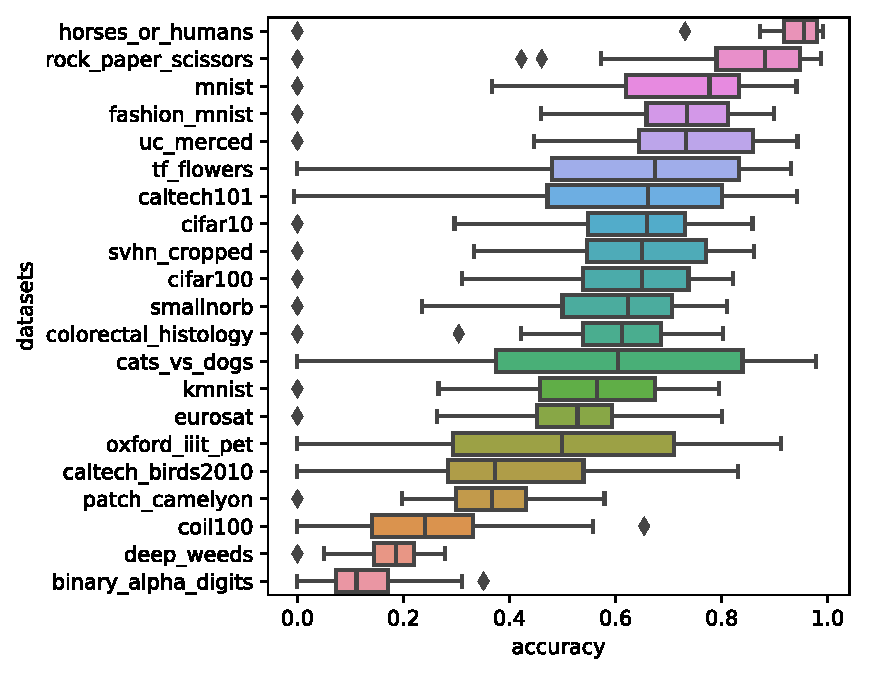
\includegraphics[width=0.95\linewidth]{../figures/dataset_results.eps} 
\end{center}
\caption{Classification accuracy of the different models across all datasets, sorted by dataset}
\label{fig:dataset_results}
\end{figure} 
%
\begin{figure}[htb]
\begin{center}
 	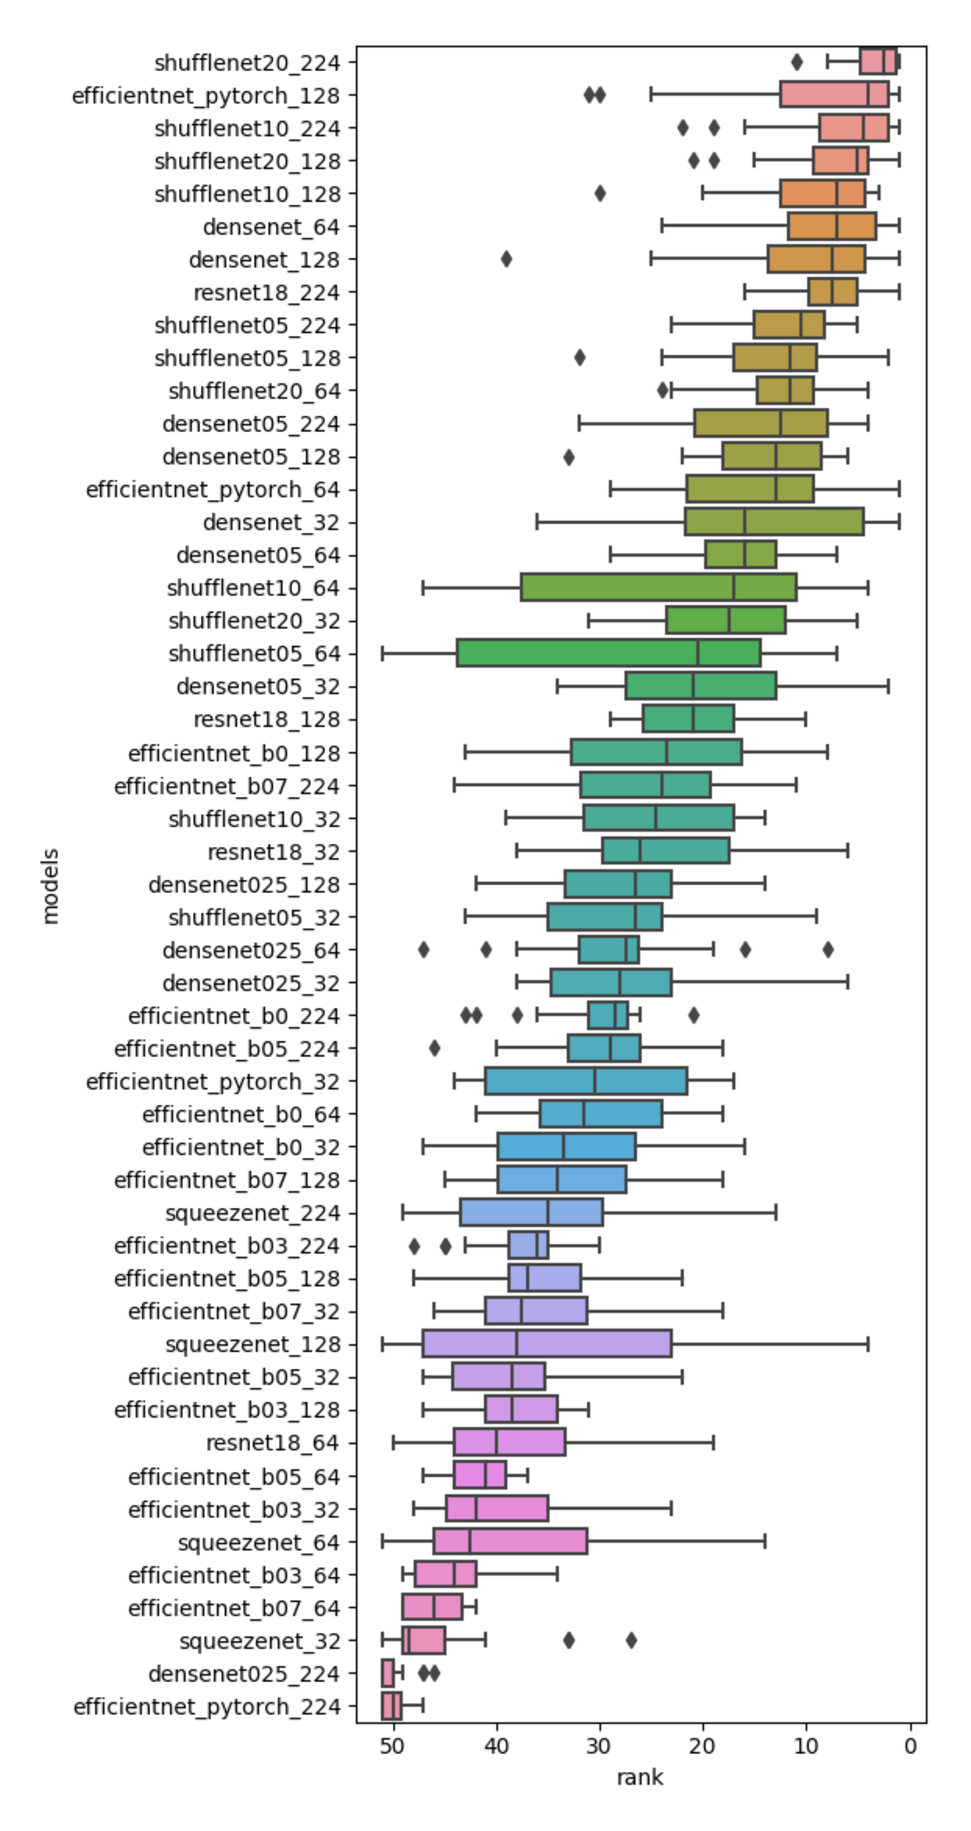
\includegraphics[width=0.95\linewidth]{../figures/rank_results.eps} 
\end{center}
\caption{Classification accuracy of the different models across all datasets, sorted by model}
\label{fig:rank_results}
\end{figure} 
%
In addition, multiple optimization runs find an optimal meta-feature vector and a reasonable distance measure while keeping the configuration space $\Theta$ small: Being reasonably small and fast, a ResNet18 network pretrained on ImageNet serves as basis to generate the meta-feature vector $\mathbf{m}(t_j)$. However, using the output of the second last layer yields consistently better results than the last output and is therefore chosen.

The following parameters have been optimized with BOHB for the different approaches: 

First approach (KMeans):
\begin{itemize}
\item Number of clusters: 5 - 40
\item Number of different initializations: 10 - 30
\item Maximum number of iterations per run: 100 - 500
\end{itemize}

Second approach (MLP with maj. vote):
\begin{itemize}
\item Train batch size: 1/2/4/8/16/32/64/128/256/512/1024
\item Neurons per layer: 16/32/64/128/256/512/1024
\item Learning rate: 1e-5 - 1e-2
\item Dropout rate: 0 - 0.8
\end{itemize}

Third approach (MLP with precalculation):
%
\begin{itemize}
\item Train batch size: 1/2/4/8/16/32/64/128/256/512/1024
\item Neurons per layer: 16/32/64/128/256/512/1024
\item Learning rate: 1e-5 - 1e-2
\item Dropout rate: 0 - 0.8
\item p-quantile: 0 - 0.4
\item (Do not) use mean, median, standard deviation, variance, skewness, kurtosis
\end{itemize}
%

Final results of the different approaches are shown in Fig.~(TODO): For every test data. Every plot shows the ALC according to Eq.  
\begin{figure}[!ht]
   \begin{minipage}{\linewidth}
   \centering
   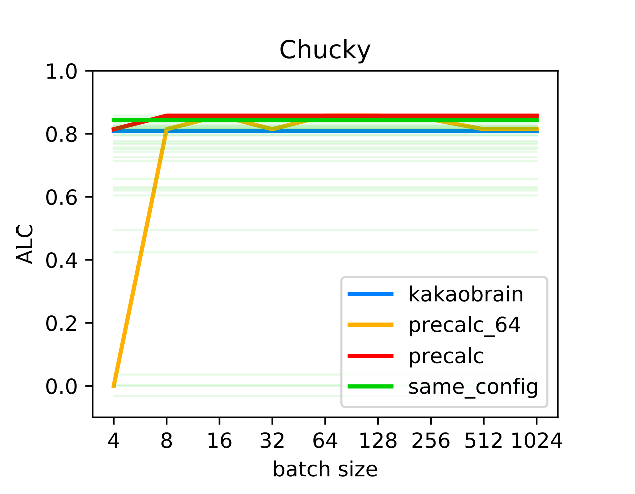
\includegraphics[width=.45\linewidth]{../figures/Chucky.eps}
   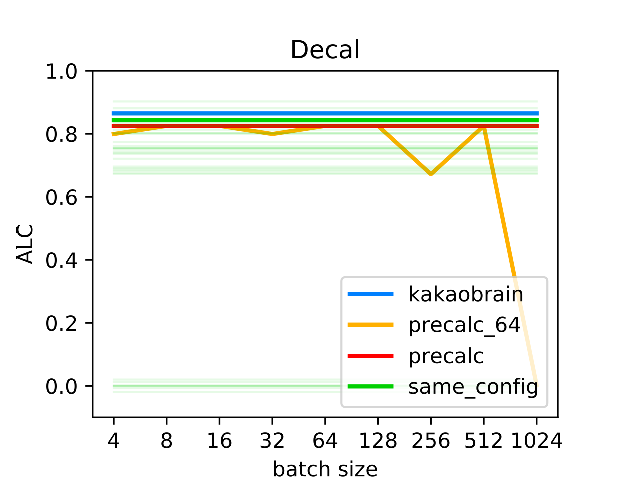
\includegraphics[width=.45\linewidth]{../figures/Decal.eps}\\
	 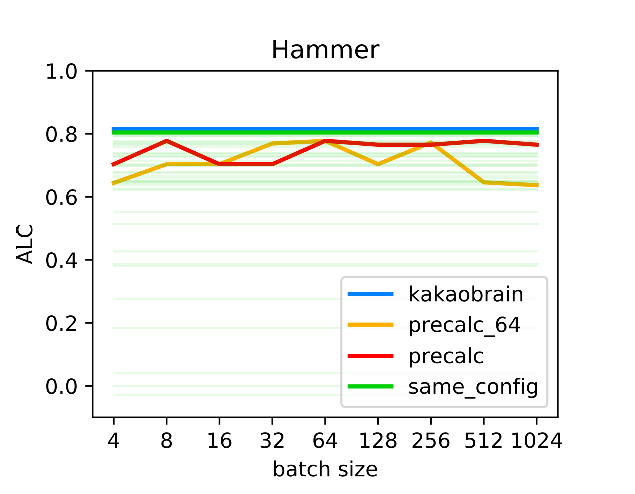
\includegraphics[width=.45\linewidth]{../figures/Hammer.eps}
   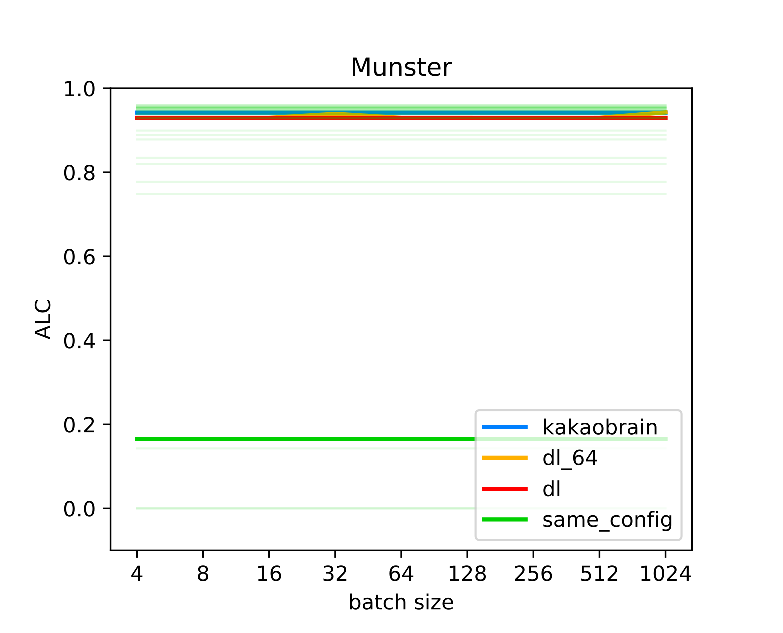
\includegraphics[width=.45\linewidth]{../figures/Munster.eps}\\
	 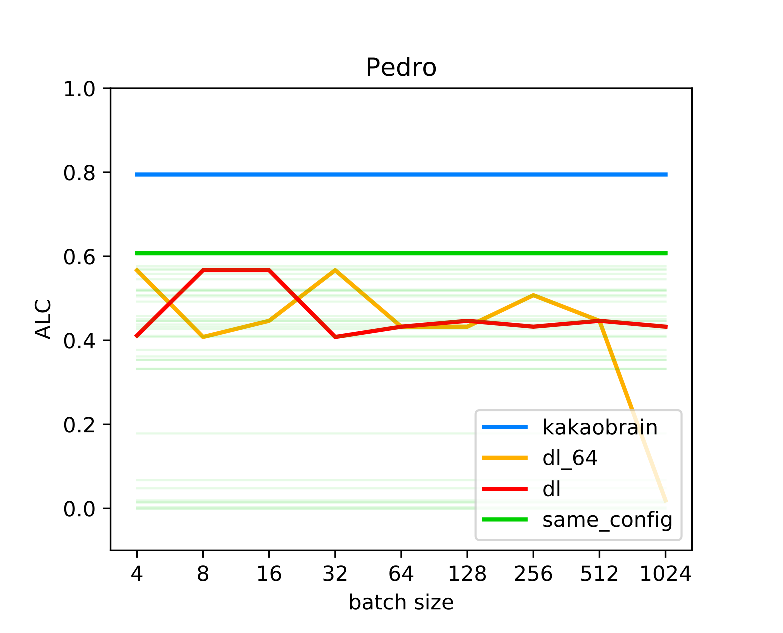
\includegraphics[width=.45\linewidth]{../figures/Pedro.eps}
   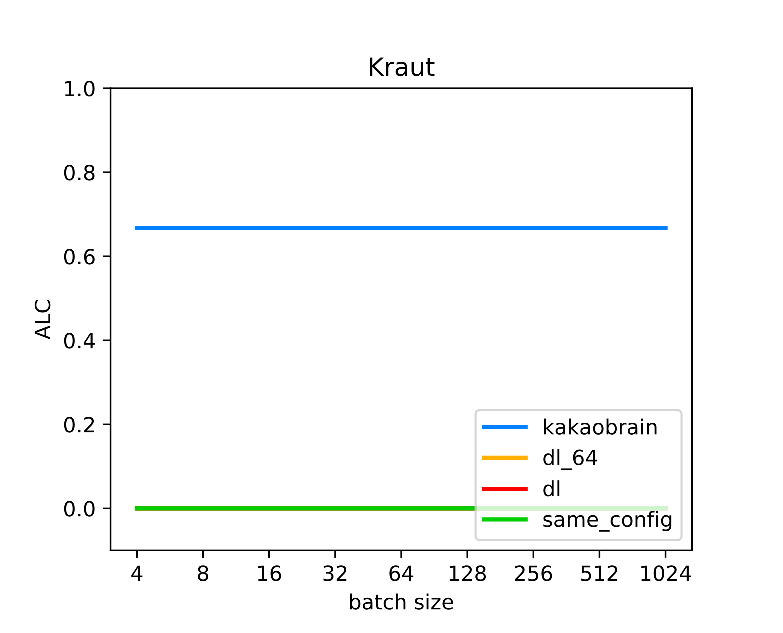
\includegraphics[width=.45\linewidth]{../figures/Kraut.eps}\\
   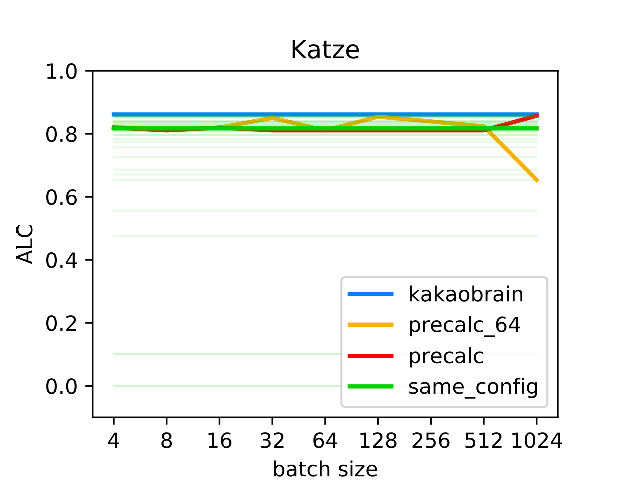
\includegraphics[width=.45\linewidth]{../figures/Katze.eps}
   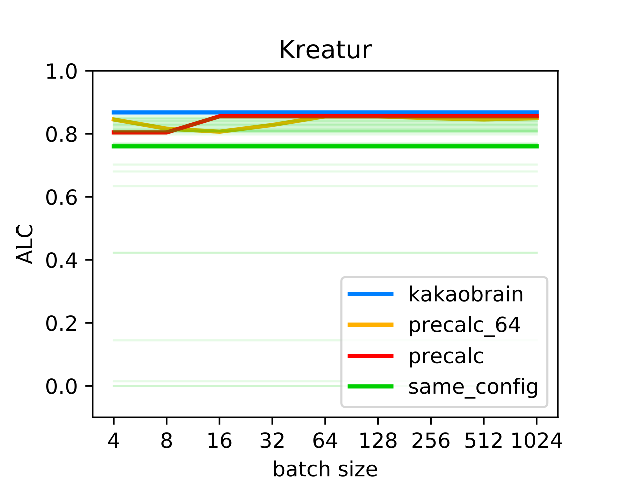
\includegraphics[width=.45\linewidth]{../figures/Kreatur.eps}
   \caption{TODO}
   \label{fig:results}
	 \end{minipage}
\end{figure}



Having found optimal configuration

Choosing an optimal test batch size is crucial during runtime. When being too small, not enough samples are used to calculate the mean, median, etc. Thus the classification accuracy decreases. When being too large, more samples than necessary are processed. This leads to computational overhead. Fig.~ shows the classification accuracy of the fingerprint network of all the datasets in Fig.~\ref{fig:dataset_results}. For every fixed test batch size 100 BOHB runs were performed. It is visible that the classification accuracy increases until a test batch size of 512 after which it decreases again. For the final experiments a test batch size of 32 or 64 seems to be a good compromise between speed and accuracy. 
%
\begin{figure}[htb]
\begin{center}
 	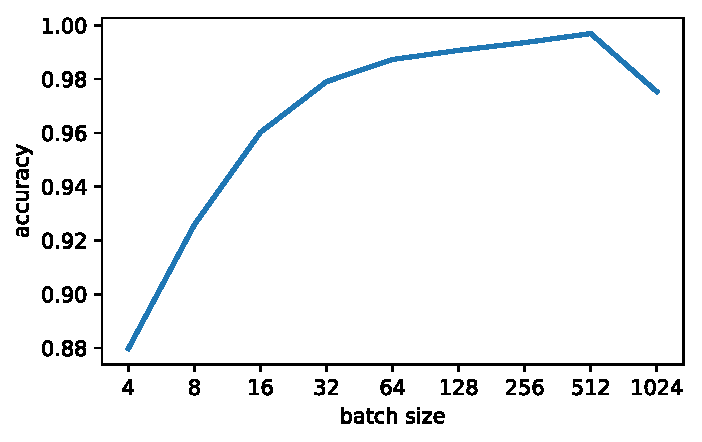
\includegraphics[width=0.7\linewidth]{../figures/batch_size_acc.eps} 
\end{center}
\caption{Classification accuracy of the fingerprint network depending on test batch size}
\label{fig:batch_size_acc}
\end{figure} 
%

If memory is limited it can be necessary to use only a reduced model portfolio instead of all models shown in Fig.~\ref{fig:rank_results}. Fig.~\ref{fig:portfolio_performance} shows the minimum/average portfolio performance across all datasets listed in Fig.~\ref{fig:dataset_results} when using only a reduced portfolio consisting of $m$ different models. The reduced portfolio is optimized for $0.5(\text{min.acc.+avg.acc.})$. One can see that a portfolio size of $m>3$ leads only to marginal improvements.
%
\begin{figure}[htb]
\begin{center}
 	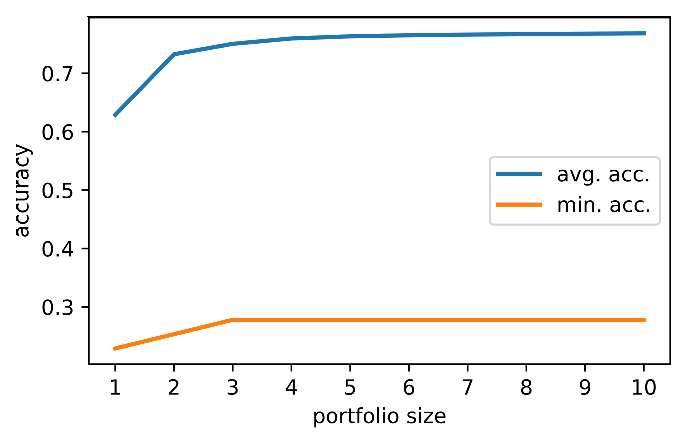
\includegraphics[width=0.7\linewidth]{../figures/portfolio_performance.eps} 
\end{center}
\caption{Portfolio performance depending on portfolio size}
\label{fig:portfolio_performance}
\end{figure} 
%


\bibliography{../bib/autodl}
\bibliographystyle{icml2018}

\end{document}


% This document was modified from the file originally made available by
% Pat Langley and Andrea Danyluk for ICML-2K. This version was created
% by Iain Murray in 2018. It was modified from a version from Dan Roy in
% 2017, which was based on a version from Lise Getoor and Tobias
% Scheffer, which was slightly modified from the 2010 version by
% Thorsten Joachims & Johannes Fuernkranz, slightly modified from the
% 2009 version by Kiri Wagstaff and Sam Roweis's 2008 version, which is
% slightly modified from Prasad Tadepalli's 2007 version which is a
% lightly changed version of the previous year's version by Andrew
% Moore, which was in turn edited from those of Kristian Kersting and
% Codrina Lauth. Alex Smola contributed to the algorithmic style files.
